\documentclass{article}
\usepackage{cite}
\usepackage[utf8]{inputenc}
\newcommand\independent{\protect\mathpalette{\protect\independenT}{\perp}}
\def\independenT#1#2{\mathrel{\rlap{$#1#2$}\mkern2mu{#1#2}}}
\title{Report for Comp Exam}
\author{Siyuan Zhao}
\date{March 2017}

\usepackage[linesnumbered,ruled]{algorithm2e}
\usepackage{amsmath, mathtools}
\usepackage{amsfonts}
\begin{document}

\maketitle

\section{Problem Setup}
Let $\mathcal{T}$ be the set of proposed interventions we wish to
consider, $X$ the set of participants, and $Y$ the set of possible
outcomes. For each proposed intervention $t \in \mathcal{T}$, let
$Y(t) \in Y$ be the potential outcome for $x$ when x is assigned to
the intervention $t$. In randomized control trial (RCT) and observed
study, only one outcome is observed for a given participant $x$; even
if the participant is given an intervention and later the other, the
participant is not in the same state.

In the binary intervention set, there are two possible interventions
$\mathcal{T} = \left \{  0, 1 \right \}$, where intervention 1 is
often referred as the "treated" and intervention 0 is the "control."
Given a sample of subjects and a treatment, each subject has a pair of
potential outcomes: $Y_i(0)$ and $Y_i(1)$, the outcomes under the
control and the treatment, respectively. Let $t$ be an indicator
variable denoting the treatment received ($t = 0$ for the control and
$t=1$ for the treatment). Only one outcome, $Y_i (Y_i=t\cdot Y_i(1) +
(1-t) \cdot Y_i(0))$, is observed for the
subject $i$.

The individual treatment effect (ITE) can be defined to
be $Y_i(1) - Y_i(0)$. The average treatment effect (ATE) is defined to
be $E[Y_i(1) - Y_i(0)]$. The ATE is the average treatment effect, at
the population level, of moving an entire population from the control
to the treatment. A related measure of treatment effect is the average
treatment effect for the treated (ATT) \cite{imbens2004}. The ATT is
defined as $E[Y(1)-Y(0) \mid t=1]$. The ATT is the average effect of
treatment on those subjects who ultimately received the treatment. In
an RCT these tow measures of treatment effects coincide because, due
to randomization, the treated population will not, on average, differ
systematically from overall population.

\subsection{Randomized Controlled Trials}
In RCTs, treatment is assigned by randomization. As a consequence of
randomization, an unbiased estimate of the ATE can be directly
computed from the data. An unbiased estimate of the ATE is
$E[Y_i(1)-Y_i(0)]=E[Y(1)] - E[Y(0)]$. This definition allows one to
define the ATE in terms of a difference in means (continuous outcomes)
or a difference in proportions (binary outcomes).

\subsection{Observational Studies}
An observational study has the same intent as a randomized experiment:
to estimate a causal effect. However, an observational study differs
from a RCT in one design issue: the use of randomization to allocate
units to treatment and control groups.

In observational studies, the treated subjects often differ
systematically from untreated subjects. In general, $E[Y(1)\mid t=1]
\neq E[Y(1)]$ holds. Thus, an unbiased estimate of the average
treatment effect cannot be obtained by directly comparing outcomes
between the two treatment groups.

\subsection{Strong Ignorability}
The treatment assignment is defined to be strongly ignorable
\cite{rosenbaum1983central} if the following two conditions hold: 1).
$(Y(1), Y(0)) \independent t\mid X$ and 2). $0 < \Pr (t=1 \mid X) <
1$. The first condition says that treatment assignment is independent
of the potential outcomes conditional on the observed baseline
covariates. The second condition says that every subject has a nonzero
probability to receive either treatment. The aforementioned first
condition is also referred to as the "no unmeasured confounders"
assumption that all variables that affect treatment assignment and
outcome have been measured.
\section{Random Causal Forest}
\cite{wager2015estimation} proposed random causal forest (RCF) to
infer treatment effect. From the conceptual point of view, trees and forests can be viewed as
nearest neighbor methods with an adaptive neighborhood metric. Given
observed independent samples $(X_i, Y_i, W_i)$, a causal tree is first
built by recursively splitting the feature space until all samples are
partitioned into a set of leaves $L$, each of which contains a few
training samples. Then, for a data point $x$, the predicted outcome $\hat{\mu}(x)$
is evaluated by identifying the leaf $L(x)$ containing $x$ and
calculating

$$\hat{\mu} = \frac{1}{\left | \left \{ i: X_i \in L(x) \right \}
  \right |} \sum_{\left \{ i: X_i \in L(x) \right \}} Y_i$$

Given a test point $x$, the closest points to $x$ are those fall in the same
leaf as it. The authors believe that the leaf is small enough that the
responses $Y_i$ are roughly identically distributed. Then the
treatment effect $\hat{\tau}$ for any $x \in L(x)$ is estimated as
following:

\begin{align} 
\hat{\tau}(x) & = \frac{1}{\left | \left \{ i: W_i=1, X_i \in L(x) \right \}
                \right |} \sum_{\left \{ i: W_i = 1, X_i \in L(x)
                \right \}} Y_i \nonumber \\
              & - \frac{1}{\left | \left \{ i: W_i=0, X_i \in L(x) \right \}
  \right |} \sum_{\left \{ i: W_i = 0, X_i \in L(x) \right \}} Y_i \label{eq:tree-treatment-effect}
\end{align}

RCF assumes that
there is overlapping in the data, i.e., for some $\epsilon > 0$ and
all $x \in \left [ 0, 1\right ]^d$,

$$\epsilon < \mathbb{P}\left [ W=1 \mid X=x \right ] < 1-\epsilon$$

This condition effectively guarantees that, for large enough $n$,
there will be enough treatment and control units near any test point
$x$ for local methods to work.

\subsection{Honest Trees and Forests}
A tree is honest if, for each training example $i$, it only uses the
response $Y_i$ to estimate the within-leaf treatment effect $\tau$
using Equation~\ref{eq:tree-treatment-effect} or
to decide where to place the splits, but not
both. \cite{wager2015estimation} proposed two causal forest algorithms
that satisfy this condition.

The first algorithm, which is called double-sample tree, achieves
honesty by dividing its training sub-sample into two halves
$\mathcal{I}$ and $\mathcal{J}$. Then, it uses the
$\mathcal{J}$-sample to place the splits, while holding out the
$\mathcal{I}$-sample to do within-leaf estimation. The details of the
algorithm is shown in Algorithm~\ref{algo:double-sample-trees}.

\LinesNumberedHidden
\begin{algorithm}[h]
  \SetKwInOut{Input}{Input}
  \Input{$n$ training examples of $(X_i, Y_i, W_i)$, where $X_i$ are
    features, $Y_i$ is the response, and $W_i$ is the treatment
    assignment. \\
    A minimum leaf size $k$.
  }

  \caption{Double-sample Causal Trees}
  \ShowLn Draw a random subsample of size $s$ from $\{1, \ldots, n\}$ without
  replacement, and then divide it into two disjoint sets of size
  $|\mathcal{I}|=\left \lfloor s/2 \right \rfloor$ and
  $|\mathcal{J}|=\left \lceil s/2 \right \rceil$ \\
  \ShowLn Grow a tree via recursive partitioning. The splits are chosen using
  any data from the $\mathcal{J}$ sample and $X$- or $W$-observations
  from the $\mathcal{I}$ sample, but without using $Y$-observations
  from $\mathcal{I}$-sample. \\
  \ShowLn Estimate leaf-wise response using only the $\mathcal{I}$-sample
  observations. \\ [1\baselineskip]

The algorithm estimates $\hat{\tau}(x)$ using
Equation~\ref{eq:tree-treatment-effect} on the $\mathcal{I}$
sample. The splitting criteria is to maximize the variance of
$\hat{\tau}(X_i)$ for $i \in \mathcal{J}$. Each leaf of the tree must
contain $k$ or more $\mathcal{I}$-sample observations of each
treatment class.
\label{algo:double-sample-trees}
\end{algorithm}
Another way to build honest trees is to ignore the outcome $Y_i$ when
placing splits, and instead first train a classification tree for the
treatment assignments $W_i$. Such propensity trees can be particularly
useful in observational studies, where we want to minimize bias due to
variation in $e(x)$. Seeking estimators that match training examples
based on estimated propensity is a longstanding idea from Propensity
Score Matching (PSM).

\LinesNumberedHidden
\begin{algorithm}[h]
  \SetKwInOut{Input}{Input}
  \Input{$n$ training examples of $(X_i, Y_i, W_i)$, where $X_i$ are
    features, $Y_i$ is the response, and $W_i$ is the treatment
    assignment. \\
    A minimum leaf size $k$.
  }
  \ShowLn Draw a random subsample $\mathcal{I} \in {1, \ldots, n}$ of
  size $|\mathcal{I}| = s$ (no replacement). \\
  \ShowLn Train a classification tree using sample $\mathcal{I}$ where
  the outcome is the treatment assignment, i.e., on the $(X_i, W_i)$
  pairs with $i \in \mathcal{I}$. Each leaf of the tree must have $k$
  or more observations of each treatment class. \\
  \ShowLn Estimate $\tau(x)$ using
  Equation~\ref{eq:tree-treatment-effect} on the leaf containing $x$.
  \caption{Propensity Trees}
\end{algorithm}
\section{Counterfactual Inference}
\cite{Johansson2016-dh} proposed Balancing Neural Networks (BNN) which
can be applied to solve the counterfactual inference problem. They
used a form of regularizer to enforce the similarity between the
distributions of representations learned for populations with
different interventions, for example, the representations for students
who received text hints versus those who received video hints.This
reduces the variance from fitting a model on one distribution and
applying it to another. Because of random assignment to the
interventions in RCTs, the distributions of the populations within
different interventions are highly likely to be identical. However, in
the observational study, we may end up with the situation where only
male students receive video hints and female students receive text
hints. Without enforcing the similarity between the distributions of
representations for male and female students, it is not safe to make a
prediction of the outcome if male students receive text hints. In
machine learning, "domain adaptation" refers to the dissimilarity of
the distributions between the training data and the test data.

In the "treated" and the "control" setting, we refer to the observed and unobserved outcomes as the factual outcome $y^F(x)$, and the counterfactual outcome $y^{CF}(x)$ respectively. In other words, when the participant $x$ is assigned to the "control" ($t = 0$), $y^F(x)$ is equal to $Y_1(x)$, and $y^{CF}(x)$ is equal to $Y_0(x)$. The other way around, $y^F(x)$ is equal to $Y_0(x)$, and $y^{CF}(x)$ is equal to $Y_1(x)$.

Given $n$ samples $\left \{ (x_i, t_i, y_i^F) \right \}_{i=1}^n$, where $y_i^F = t_i \cdot Y_1(x_i) + (1-t_i)Y_0(x_i)$, a common approach for estimating the ITE is to learn a function $f : X \times T \rightarrow Y$ such that $f(x_i, t_i) \approx y_i^F$. The estimated ITE is then:
$$\hat{ITE}(x_i) = \left\{\begin{matrix} y_i^F - f(x_i, 1-t_i), & t_i = 1.\\ f(x_i, 1-t_i) - y_i^F, & t_i = 0. \end{matrix}\right. $$

We assume $n$ samples $\left \{ (x_i, t_i, y_i^F) \right \}_{i=1}^n$ form an empirical distribution $\hat{p}^F  = \left \{ (x_i, t_i) \right \}_{i=1}^n$. We call this empirical distribution $\hat{p}^F \sim p^F$ the empirical factual distribution. In order to calculate ITE, we need to infer the counterfactual outcome which is dependent on the empirical distribution $\hat{p}^{CF}  = \left \{ (x_i, 1-t_i) \right \}_{i=1}^n$. We call the empirical distribution $\hat{p}^{CF} \sim p^{CF}$. The $p^{F}$ and $p^{CF}$ may not be equal because the distributions of the control and the treated populations may be different. The inequality of two distributions may cause the counterfactual inference over a different distribution than the one observed from the experiment. In machine learning terms, this scenario is usually referred to as domain adaptation, where the distribution of features in test data are different than the distribution of features in training data.

\begin{figure}[h]
  \centering
  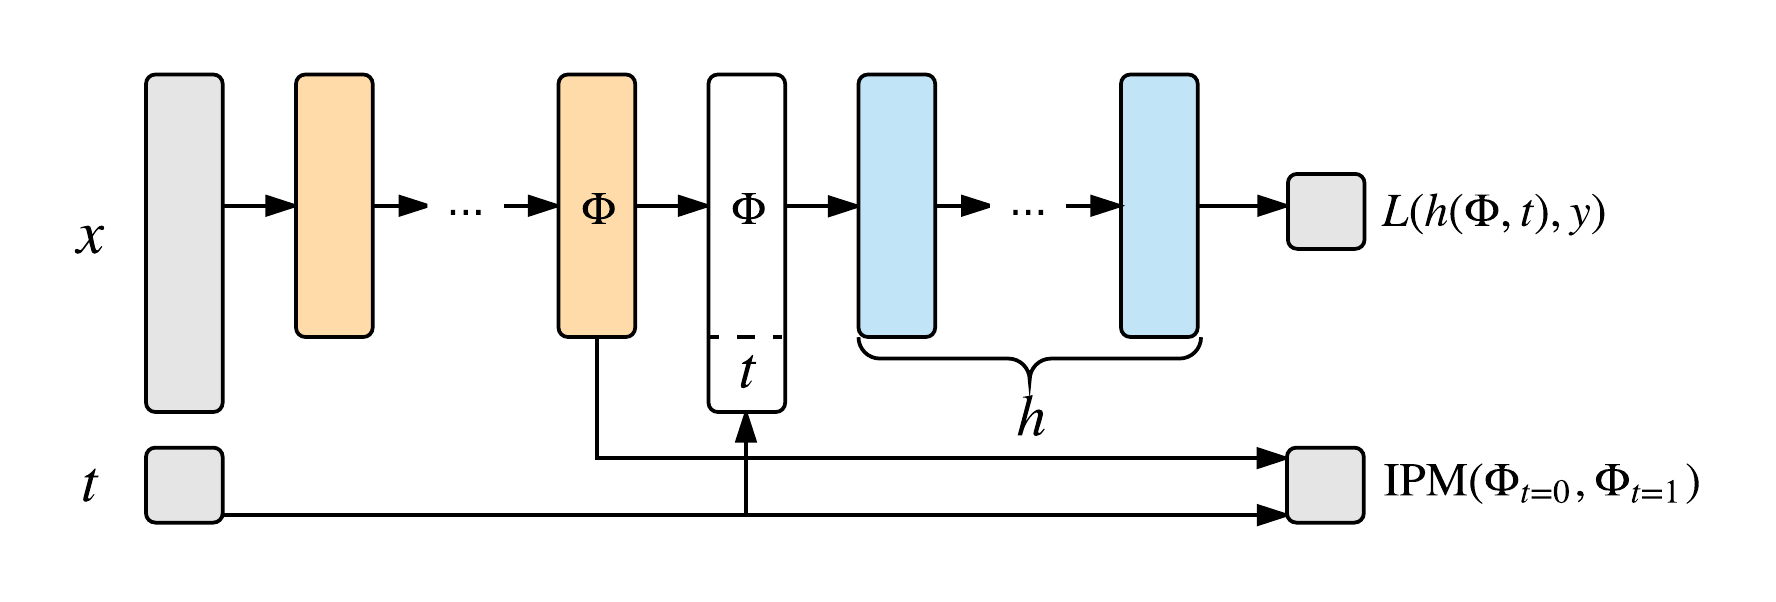
\includegraphics[width=0.95\columnwidth]{cfr.png}
  \caption{CFR for ITE estimation. $L$ is a loss function, IPM is an integral probability metric}.
  ~\label{fg:cfr-model}
\end{figure}

To learn a representation of deep features $\Phi$, the RCN uses fully connected layers with ReLu activation function, where $Relu(z) = max(0, z)$. We need to generalize from factual distribution to counterfactual distribution in the feature representation $\Phi$ to obtain accurate estimation of counterfactual outcome. The common successful approaches for domain adaptation encourage similarity between the latent feature representations w.r.t the different distributions. This similarity is often enforced by minimizing a certain distance between the domain-specific hidden features. The distance between two distributions is usually referred to as the discrepancy distance, introduced by \cite{Mansour2009-fh}, which is a hypothesis class dependent distance measure tailored for domain adaptation. 

In this paper we use an Integral Probability Metric (IPM) measure of distance between two distributions $p_0 = p(x|t = 0)$, and $p_1 = p(x|t = 1)$, also known as the control and treated distributions. The IPM for $p_0$ and $p_1$ is defined as
$$\mathrm{IPM}_{\mathcal{F}}(p_0, p_1) := \sup_{f\in \mathcal{F}} \left |\int_S f dp_0 -\int_S f d p_1 \right |,$$

where $\mathcal{F}$ is a class of real-valued bounded measurable functions on $S$. 

The choice of functions is the crucial distinction between IPMs \cite{Sriperumbudur2009-pf}. Two specific IPMs are used in our experiments: the Maximum Mean Discrepancy (MMD), and the Wasserstein distance. $\mathrm{IPM}_{\mathcal{F}}$ is called MMD, when $\mathcal{F} = \left \{ f : \left \| f \right \| _\mathcal{H}\leq 1\right \}$, where $\mathcal{H}$ represents a reproducing kernel Hilbert space (RKHS) with $k$ as its reproducing kernel. In other words, the family of norm-1 reproducing kernel Hilbert space (RKHS) functions lead to the MMD. The family of 1-Lipschitz functions $\mathcal{F} = \left \{ f:\left \| f\right \|_L \leq 1 \right \}$, where $\left \| f\right \|_L$ is the Lipschitz semi-norm of a bounded continuous real-valued function $f$, make IPM the Wasserstein distance. Both the Wasserstein and MMD metrics have consistent estimators which can be efficiently computed in the finite sample case \cite{Sriperumbudur2012-sz}. The important property of IPM is that $$p_0 = p_1~\mathrm{iff}~ \mathrm{IPM}_{\mathcal{F}}(p_0, p_1) = 0.$$

The representation with reduction of the discrepancy between the control and the treated populations helps the model to focus on balancing features across two populations when inferring the counterfactual outcomes. For instance, if in an experiment, almost no male student ever received intervention A, inferring how male students would react to intervention A is highly prone to error and a more conservative use of the gender feature might be warranted.

\section{Individualized Treatment Rules}
In experiments, we observe a triplet $(\mathbf{x}, t, y)$ from each
participant, where $\mathbf{x}=(x_1, x_2, \ldots, x_n)^T \in
\mathcal{X}$ denotes the participant's covariates, $t \in \mathcal{T}
= {-1,1}$ denotes the treatment assignment, and $y \in Y$ is the
observed outcome, also called the "reward" in the literature on
reinforcement learning. Note that $t=-1$ means the control in the
context of ITR. Let $p(t|x)$ be the probability of assigning the participant
with covariates $\mathbf{x}$ to the intervention $t$.

An individual treatment rule (ITR) $d: X \rightarrow \mathcal{T}$ is a deterministic decision
rule from subject $x$ into the intervention space $\mathcal{T}$. The
value of $d$ satisfies
$$V(d) = E \left [ \frac{y}{p(t|x)}\mathbb{I}_{t=d(\mathbf{x})}\right
],$$
where $\mathbb{I}(\cdot)$ is an indicator function. An optimal ITR, $d^{*}$, is a rule that has the maximal value such
that,

$$d^{*} \in \operatorname*{arg\,max}_d V(d).$$
Finding $d^{*}$ is equivalent to minimizing the following equation:
\begin{equation} \label{eq:d_min}
d^{*} \in \operatorname*{arg\,min}_d E \left [
  \frac{y}{p(t|x)}\mathbb{I}_{t \neq d(\mathbf{x})}\right
]
\end{equation}

Assume that the observed data $\left \{
  (\mathbf{x}_i,t_i,y_i),~i=1,\ldots , n \right \}$ are collected
independently. For any decision function $f(\mathbf{x})$, let
$d_f(\mathbf{x}) = sign(f(\mathbf{x}))$ be the associated rule, where
$sign(u) = 1$ for $u > 0$ and $-1$ otherwise. The particular choice of
the value of $sign(0)$ is not important. With the observed data, the
weighted classification error in Equation \ref{eq:d_min} can be approximated by
the empirical risk

\begin{equation} \label{eq:d_empirical_min}
  \frac{1}{n}\sum_{i=1}^{n}\frac{y_i}{p(t_i|x_i)}\mathbb{I}_{t_i \neq
    d_f(\mathbf{x_i})} .
\end{equation}

\cite{Qian2011-vz} proposed a two-step procedure that first estimates
a conditional mean for the outcome and then determines the treatment
rule by comparing the conditional means across various treatment.

In contrast, outcome weighted learning (OWL) is proposed by
\cite{zhao2012estimating} using the hinge loss function and the
regularization technique. In other words, instead of minimizing
Equation~\ref{eq:d_empirical_min}, OWL aims to minimize

\begin{equation}
  \frac{1}{n}\sum_{i=1}^{n}\frac{y_i}{p(t_i|x_i)}(1-t_if(\mathbf{x}_i))_{+}+\lambda\left
    \| f \right \|^2 ~\label{eq:d_owl_empirical_min},
\end{equation}
where $(u)_+=\max(u,0)$ is the positive part of $u$, $\left \| f
\right \|$ is some norm for $f$, and $\lambda$ is a tuning parameter
controlling the trade-off between empirical risk and complexity of the
decision function $f$.

\cite{Zhou_undated-ps} pointed out that decision rule in
Equation~\ref{eq:d_owl_empirical_min} is
affected by a simple shift of the outcome $Y$ and proposed Residual
weighted learning (RWL) to relieve this issue. The idea behind RWL is
to introduce a function $g$ to reduce the variance of
$\frac{y-g(\mathbf{x})}{p(t|\mathbf{x})}\mathbb{I}_{t \neq
  d(\mathbf{x})}$ and a reasonable candidate of $g$ is
\begin{equation}
  g^{*}(\mathbf{x}) = \frac{\mathbb{E}(y|\mathbf{x},
    t=1)+\mathbb{E}(y|\mathbf{x}, t=-1)}{2} = \mathbb{E} \left (
    \frac{y}{2p(t, \mathbf{x})} | \mathbf{x} \right ).~\label{eq:g-choice}
\end{equation}

RWL thus is to minimize the following empirical risk:
\begin{equation}
   \frac{1}{n}\sum_{i=1}^{n}\frac{y_i-\hat{g}^{*}(\mathbf{x}_i)}{p(t_i|\mathbf{x_i})}\mathbb{I}_{t_i \neq
    d_f(\mathbf{x_i})}
  ~\label{eq:rwl-risk}
\end{equation}
where $\hat{g}^{*}$ is an estimate of $g^{*}$. For simplicity, let
$\hat{r}_i = y_i - \hat{g}^{*}(\mathbf{x}_i)$. As in OWL,
\cite{Zhou_undated-ps} consider a surrogate loss function $T$ to replace
the 0-1 loss in Equation~\ref{eq:rwl-risk}. The non-convex loss $T$
has the following form:
\begin{equation}
T(u) =  \left\{\begin{array}{ll}
 0 & \mathrm{if} \: u \geq 1, \\ 
 (1-u)^2 & \mathrm{if} \: 0 \leq u < 1, \\ 
 2-(1+u)^2 & \mathrm{if} \: -1 \leq u < 0, \\ 
 2 & \mathrm{if} \: u < -1
\end{array}\right.
\end{equation}
It is called the smoothed ramp loss in \cite{Zhou_undated-ps}. By
incorporating the regularization, RWL is eventually aimed to minimize
the following empirical risk:
\begin{equation}
    \frac{1}{n}\sum_{i=1}^{n}\frac{\hat{r}_i}{p(t_i|x_i)}T(t_if(\mathbf{x}_i))_{+}+\lambda\left
    \| f \right \|^2 ~\label{eq:d_owl_empirical_min},
\end{equation}
where $\left \| f \right \|$ is the norm for $f$, and $\lambda$ is a
tuning parameter.
\section{Bayesian Optimization}
Bayesian optimization is a sequential model-based approach for global
optimization of an unknown objective function $f$. The problem can be
mathematically expressed as:

\begin{equation}
  \mathbf{x}^* = \underset{\mathbf{x} \in \mathcal{X}}{\mathrm{arg \,
      max} \, f(\mathbf{x})}
\end{equation}
where $\mathcal{X}$ is the design space of interest. Since the objective function is unknown, the Bayesian
strategy is to treat it as a random function and place a prior over it. The prior captures our beliefs about the behaviour of the
function. After gathering the function evaluations, which are treated
as data, the prior is updated to form the posterior distribution
over the objective function. Equipped with the posterior distribution,
an acquisition function $\alpha: \mathcal{X} \rightarrow \mathbb{R}$
is induced to determines what the
next query point should be. The acquisition function leverages the
uncertainty in the posterior to trade off between the exploration and
the exploitation. Examples of acquisition functions includes
probability of improvement, expected improvement, Bayesian expected
losses, upper confidence bounds (UCB), Thompson sampling and mixtures
of these. They all trade-off exploration and exploitation so as to
minimize the number of function queries. As such, Bayesian
optimization is well suited for functions that are very expensive to evaluate.

In this setting, Bayesian optimization is considered as a sequential
search algorithm which, at round $n$, selects a query point
$\mathbf{x}_{n+1}$ at which to evaluate $f$ and observe
$y_{n+1}$. After $N$ queries, the algorithm produces the best estimate
$\bar{\mathbf{x}}_N$. Under the context of multi-armed bandit
problems, function $f$ is the reward function.
  
In summary, Bayesian optimization is the combination of two main
components: a surrogate probabilistic model which captures our beliefs
about the behavior of the unknown objective function and observed
information, and an acquisition function which performs the selection
of the optimal sequence of queries based on the previous model.

The Gaussian process (GP) is the most popular model due to
its accuracy, robustness and flexibility, because Bayesian
optimization is mainly usesd in blck-box scenarios. The range of
applicaility of a Gaussian process is defined by its kernel function,
which sets the family of functions that is able to represent through
the reproducing kernel Hilbert space (RKHS). In BO, attributes of the
GP such as mean and variance are used to sample successive points. It
is suitable for situations where cost function is costly to evaluate
and MCMC techniques would not work.

\begin{algorithm}[h] \label{algo:bo}
  \SetKwInOut{Input}{Input}
  \Input{$n$ observations $\mathcal{D}=\{ (\mathbf{x}_i,
    y_i)\}_{i=1}^n$ from objective function $f$}

 \caption{Bayesian optimization with Gaussian process}
 \For{$t = n+1,n+2,\ldots$} {
   select new $\mathbf{x}_{t}$ by maximizing acquisition function
   $\alpha$
   $$
     \mathbf{x}_{t} = \underset{\mathbf{x}}{\mathrm{arg \, max}} \, \alpha(\mathbf{x};\mathcal{D})
     $$\\
     query objective function to observe $y_{t} =
     f(\mathbf{x}_{t})$ \\
     augment data $\mathcal{D}=\{ \mathcal{D},
     (\mathbf{x}_{t}, y_{t}) \}$\\
     update statistical model
 }
\end{algorithm}

\subsection{Thompson Sampling}
Thompson sampling for Beta-Bernoulli bandit perhaps is the simplest non-trivial multi-armed
bandit strategy in Bayesian optimization. Bernoulli bandit problem is
the bandit problem when the rewards are either 0 or 1, and for arm $i$
the probability of success (reward=1) is $\mu_i$. The Thompson
sampling maintains Bayesian priors on the Bernoulli means
$\mu_i$'s. Beta distribution turns out to be a very convenient choice
of priors for Bernoulli rewards. The pdf of $\mathrm{Beta}(\alpha,
\beta)$ with parameters $\alpha > 0, \beta > 0$ is given by
\begin{equation}
  f(x;\alpha, \beta) = \frac{\Gamma(\alpha + \beta)}{\Gamma(\alpha)\Gamma(\beta)}x^{\alpha-1}(1-x)^{\beta-1}.
\end{equation}

The mean of $\mathrm{Beta}(\alpha,\beta)$ is $\alpha / (\alpha +
\beta)$; and higher the $\alpha, \beta$, tighter is the concentration
of $\mathrm{Beta}(\alpha,\beta)$ around the mean. If the prior
for each arm is a $\mathrm{Beta}(\alpha,\beta)$ distribution, then
after observing a Bernoulli trial, the posterior distribution is
simply $\mathrm{Beta}(\alpha + 1,\beta)$ or
$\mathrm{Beta}(\alpha,\beta +1)$, depending on whether the trial
resulted in a success or failure, respectively. Thompson sampling then
samples from these posterior distributions across all arms and chooses
the arm with largest sample value. This procedure is summarized in
Algorithm~\ref{algo:thompson-sampling}.

\begin{algorithm}[h] \label{algo:thompson-sampling}
  \SetKwInOut{Input}{Input}
  \Input{$\alpha, \beta$: hyperparameters of the beta prior}

  \caption{Thompson sampling for Beta-Bernoulli bandit}
  Initialize $n_{a,0}=n_{a,1}=i=0$ for all $K$ arms $a$ \\
  \Repeat{stopping criterion reached} {
    \For{$a = 1,\ldots, K$}{
      $w_a \sim \mathrm{Beta}(\alpha + n_{a,1}, \beta + n_{a,0})$
    }
    $a_i = \underset{a}{\mathrm{arg\, max}}\, w_a$ \\
    Observe $y_i$ by pulling arm $a_i$ \\
    \eIf{$y_i = 0$}{
      $n_{a_i,0} = n_{a_i,0} + 1$
      
    }{
      $n_{a_i,1} = n_{a_i,1} + 1$
    }
    $i = i + 1$ \\
 }
\end{algorithm}

\subsection{Choice between function predictor and multi-armed bandit algorithm}
In many applications, the designs available to the experimenter have
components that can be varied independently. For example, in designing
an advertisement, one has choices such arkwork, font style, and
size. If there are five choices for each, the total number of possible
configurations is 125.

In general, this number grows combinatorially in the number of
components. This presents challenges for approaches such as the independent
Thompson sampling, since the Thompson sampling models the arms as independent, which will lead
to strategies that must try every option at least once. This rapidly
becomes infeasible in the large spaces of real-world problems.

Even if the total number of possible design configuration is
relatively small, it is still challenging for multi-armed bandit
algorithms when the number of available subjects is limited for these
algorithms to figure out the optimal arm.

To alleviate this issue, a commonly used approach is to learn a
function, whose input is a feature vector of the arm and output is
associated reward of the arm, capturing dependence between the arms. Assume that each possible arm $a$ has an
associated feature vector $\mathbf{x}_a\in \mathbb{R}^d$. The expected
reward of each arm can be expressed as a function of this feature
vector, such as $f(a) = f(\mathbf{x}_a)$. The goal is to learn this
function $f:\mathbb{R}^d \rightarrow \mathbb{R}$ from the experiment
data in order to choose the arm with the highest reward among all
possible arms.

\section{Online Learning vs. Batch Learning}
In machine learning, online machine learning is a method of machine
learning in which data becomes available in a sequential order and is
used to update our best predictor for future data at each step, as
opposed to batch learning techniques which generate the best predictor
by learning on the entire training data set at once.

\subsection{Sequential method}
The sequential approach is independent of the choice of prior and of
the likelihood function and depends only on the assumption of i.i.d
data. Sequential methods make use of observations one at a time, or in
small batches, and then discard them before the next observations are
used. They can be used, for example, in real-time learning scenarios
where a steady stream of data is arriving, and predictions must be
made before all of the data is seen. Because they do not require the
whole data set to be stored or loaded into memory, sequential methods
are also useful for large data sets.

\section{Semi-Supervised Learning}
In the context of semi-supervised learning, the training data consists
of $l$ labeled instances $\left \{ (\mathbf{x}_i, y_i)
\right \}_{i=1}^{l}$ and $u$ unlabeled instances $\left \{ (\mathbf{x}_j)
\right \}_{j=l+1}^{l+u}$, often with $u \ll l$. The goal of
semi-supervised learning is to learn a model with better performance
from the training data than from labeled data alone. It is known that
the labeled data can be hard and expensive to obtain since labels may
require human experts, and the unlabeled data is often cheap in large
quantity.

\begin{figure}[h] \label{fg:ssl_model}
  \centering
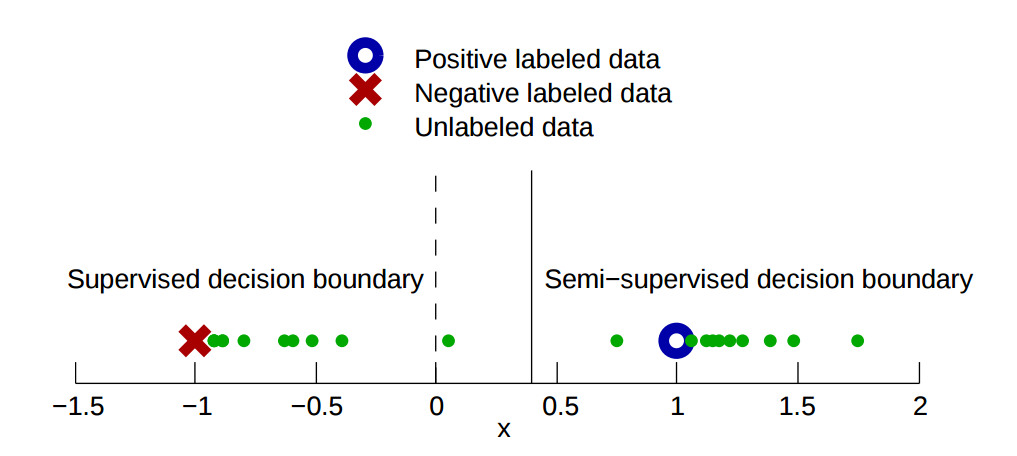
\includegraphics[width=10cm]{ssl.png}
\end{figure}

Co-training \cite{blum1998combining} is a semi-supervised learning technique that requires two
views of the data. It assumes that each example is described using two
different feature sets that provide different, complementary
information about the instance. Co-training first learns a separate
classifier for each view using any labeled examples. The most
confident predictions of each classifier on the unlabeled data are
then used to iteratively construct additional labeled training
data. The details of co-training algorithm is described in Algorithm~\ref{algo:co-training}.
\begin{algorithm}[h] \label{algo:co-training}
  \SetKwInOut{Input}{Input}
  \Input{labeled data $\left \{ (\mathbf{x}_i, y_i)
\right \}_{i=1}^{l}$, unlabeled data $\left \{ \mathbf{x}_j
\right \}_{j=l+1}^{l+u}$ \\
each instance has two views $\mathbf{x}_i=\left [ \mathbf{x}_i^{(1)},
  \mathbf{x}_i^{(2)} \right ]$ \\
and a learning speed $k$
}
Let $L_1 = L_2 = \left \{ (\mathbf{x}_1, y_1), \ldots, (\mathbf{x}_l, y_l)
\right \}.$ \\
\Repeat {unlabeled data is used up}{
  Train view-1 $f^{(1)}$ from $L_1$, view-2 $f^{(2)}$ from $L_2$ \\
  Classify unlabeled data with $f^{(1)}$ and $f^{(2)}$ separately. \\
  Add $f^{(1)}$'s top $k$ most-confident predictions $(\mathbf{x},
  f^{(1)}(\mathbf{x}))$ to $L_2$ \\
  Add $f^{(2)}$'s top $k$ most-confident predictions $(\mathbf{x},
  f^{(2)}(\mathbf{x}))$ to $L_1$ \\
  Remove these from the unlabeled data.
}

\caption{Co-training Algorithm for Semi-Supervised Learning}
\end{algorithm}

There are three important assumptions which guarantee the performance of
co-training algorithm: 1). feature split $x=[x^{(1)};x^{(2)}]$
exists; 2). $x^{(1)}$ or $x^{(2)}$ alone is sufficient to train a good
classifier; 3). $x^{(1)}$ and $x^{(2)}$ are conditionally independent
given the class.

\section{Propensity Score Matching}
A propensity score \cite{rosenbaum1983central} is the probability of a unit (e.g., student,
classroom, school) being assigned to a particular treatment given a
set of observed covariates. Propensity scores are used to reduce
selection bias by equating groups based on these covariates.

Suppose that we have a binary treatment $T=\{0,1\}$, an outcome $Y$, and
background variables $X$. The propensity score is defined as the
conditional probability of treatment given background variables:
$$p(x):= \Pr(T=1 \mid X=x)$$
Let $Y(0)$ and $Y(1)$ denote the potential outcomes under the control
and the treatment, respectively.

The actual propensity score in observational experiments is
unknown and it can be estimated using statistical or machine
learning models from the experiment data. The most commonly used model
is a logistic regression model, in which treatment assignment $T$ is
regressed on background variables $X$. Behind logistic regression, the
use of bagging or boosting \cite{Lee2010-zr}, tree-based model
(Propensity trees) and causal random forests
\cite{wager2015estimation}, and neural networks
\cite{setoguchi2008evaluating} have been proposed to estimate the
propensity score.

The purpose of Propensity score matching (PSM) is to form matched sets of treated and
untreated subjects who share a similar value of the propensity
score. PSM allows one to estimate the average treatment effect for the
treated (ATT) \cite{imbens2004nonparametric}. The ATT is the average effect of treatment on those
subjects who ultimately receive the treatment. The most common
implementation of PSM is one-to-one or pair matching, in which pairs
of the control and the treated subjects are formed, such that matched
subjects have similar values of the propensity score. Once a matched
sample has been formed, the treatment effect can be estimated by
directly comparing outcomes between treated and untreated subjects in
the matched sample. If the outcome is continuous, the effect of
treatment can be estimated as the difference between the mean outcome
for treated subjects and the mean outcome for untreated subjects in
the matched sample. If the outcome is binary, the effect of treatment
can be estimated as the difference between the proportion of subjects
experiencing the event in each of the two groups (the treated
vs. the control) in the matched sample. In summary, the analysis of a propensity score matched sample can mimic that of an
RCT: one can directly compare outcomes between the treated and the control
subjects within the propensity score matched sample. 


The possibility of bias arises because the apparent difference in outcome between these two groups of units may depend on characteristics that affected whether or not a unit received a given treatment instead of due to the effect of the treatment per se. In randomized experiments, the randomization enables unbiased estimation of treatment effects; for each covariate, randomization implies that treatment-groups will be balanced on average, by the law of large numbers. Unfortunately, for observational studies, the assignment of treatments to research subjects is typically not random. Matching attempts to mimic randomization by creating a sample of units that received the treatment that is comparable on all observed covariates to a sample of units that did not receive the treatment.

\section{Gaussian Processes in Bandit Settings}
Bayesian algorithms do not attempt to identify ‘best-fit’ models of the data (or similarly, make 'best guess' predictions for new test inputs). Instead, they compute a posterior distribution over models (or similarly, compute posterior predictive distributions for new test input). These distributions provide a useful way to quantify our uncertainty in model estimates, and to exploit our knowledge of this uncertainty in order to make more robust predictions on new test points.

The Gaussian process is the extension of multivariate Gaussian to infinite-sized collections of real-valued variables. In particular, this extension will allow us to think of Gaussian processes as distributions not just over random vectors but in fact distributions over random functions.

The Gaussian process $\mathrm{GP}(\mu_0,k)$ is a non-parametric model
that is fully characterized by its prior mean function $\mu_0 :
\mathcal{X}\rightarrow \mathbb{R}$ and its positive-definite kernel,
or covariance function, $k: \mathcal{X} \times \mathcal{X} \rightarrow
\mathbb{R}$.

Let $\mathcal{D}_n = \left \{( \mathbf{x}_i, y_i \right )\}$ denote a
set of $n$ observations and $\mathbf{x}$ denote the arbitrary test
point. The random variable $f(\mathbf{x})$ is also a GP distribution
conditioned on observations $\mathcal{D}_n$ with following mean
$\mu_n(\mathbf{x})$ and variance $\sigma_n^2(\mathbf{x})$:
\begin{align}
 \mu_n(\mathbf{x}) &= \mu_0(\mathbf{x}) +
                     \mathbf{k}(\mathbf{x})^T(\mathbf{K}+\sigma^2\mathbf{I})^{-1}(\mathbf{y}-\mathbf{m})
  \\
  \sigma_n^2(\mathbf{x}) &= k(\mathbf{x}, \mathbf{x}) -
                           \mathbf{k}(\mathbf{x})^T(\mathbf{K}+\sigma^2\mathbf{I})^{-1}\mathbf{k}(\mathbf{x})
\end{align}
where $m_i := \mu_0(\mathbf{x}_i)$, $K_{i,j} := k(\mathbf{x_i, x_j})$,
and $\mathbf{k}(\mathbf{x})$ is a vector of covariance terms between
$\mathbf{x}$ and $\mathbf{x}_{1:n}$.

The posterior mean and variance evaluated at any point $\mathbf{x}$
represent the model's prediction and uncertainty in the objective
function at the point $\mathbf{x}$. In order to apply GP under the
setting of multi-armed bandit, we need a acquisition function to select
the next query point given the posterior model. The acquisition
function should be carefully design to trade off exploration of the
search area and exploitation of current promising areas.

\subsection{GP-UCB}
To decrease uncertainty globally, one strategy could be to pick the
point which maximums the variance $\mathbf{x}_{n+1}=
\underset{\mathbf{x} \in
  D}{\mathrm{arg\,max}}~\sigma_n(\mathbf{x})$. However, this strategy
is not well suited for multi-armed bandit problem since it can be
wasteful. Another idea is to
select the point which maximizes the expected reward given the
posterior model $\mathbf{x}_{n+1}=
\underset{\mathbf{x} \in
  D}{\mathrm{arg\,max}}~\mu_n(\mathbf{x})$. However, this idea is too
greedy and tends to end up with a local optima. To balance exploration
and exploitation, a combined strategy is to choose
\begin{equation}
  \mathbf{x}_{n+1} = \underset{\mathbf{x} \in D}{\mathrm{arg \,
      max}}\,\mu_n(\mathbf{x})+\beta_n \sigma_n(\mathbf{x}),
\end{equation} \label{eq:gp-ucb-query}
where $\beta_n$ are constants. There are theoretically motivated
guidelines for setting and scheduling the hyperparameter $\beta_n$ to
achieve optimal regret.

Since Equation~\ref{eq:gp-ucb-query} is an upper confidence bound of
the marginal posterior $P(f(\mathbf{x})|\mathbf{y}_n)$, a natural
interpretation of this strategy is that it selects the point
$\mathbf{x}$ such that $f(\mathbf{x})$ is a reasonable upper bound on
$f(\mathbf{x})$. This algorithm is called Gaussian process upper
confidence bound (GP-UCB), introduced by \cite{Srinivas2010-hi}. The
GP-UCB selection rule is motivated by the UCB algorithm for the
classical multi-armed bandit problem.

\subsection{Contextual GP-UCB}
Motivated by GP-UCB algorithm mentioned above, \cite{Krause2011-sb}
extended the generalization of this algorithm by incorporating
contextual information
\begin{equation}
  \mathbf{x}_{n+1} = \underset{\mathbf{x} \in D}{\mathrm{arg \,
      max}}\,\mu_n(\mathbf{x}, \mathbf{z}_n)+\beta_n
  \sigma_n(\mathbf{x}, \mathbf{z}_n),
\end{equation} \label{eq:cgp-ucb-query}
where $z_n \in Z$ is the contextual information from a set $Z$ of
contexts, $\mu_n(\cdot)$ and $\sigma_n^2(\cdot)$ are the posterior mean
and variance of the GP conditioned on observations $\mathcal{D}_n =
\left \{( \mathbf{x}_i, \mathbf{z}_i, y_i \right )\}.$ The authors
called the selection rule the contextual Gaussian process UCB
algorithm (GCP-UCB).

To derive the kernel $k$ on the product space $Z\times X$ of contexts and
actions, a natural approach to start with kernel functions $k_Z:
Z\times Z \rightarrow \mathbb{R}$ and $k_X:X \times X \rightarrow
\mathbb{R}$ on the space of contexts and actions. \cite{Krause2011-sb}
proposed two possibilities of constructing composite kernel $k$ from
context kernel $k_Z$ and action kernel $k_X$. One is to calculate a
product kernel $k=k_Z\otimes k_X$, by setting
\begin{equation}
  (k_Z\otimes k_X)((\mathbf{z}, \mathbf{x}),(\mathbf{z}^{\prime},
  \mathbf{x}^{\prime})) = k_Z(\mathbf{z}, \mathbf{z}^{\prime})k_X(\mathbf{x}, \mathbf{x}^{\prime}).
\end{equation}

An alternative is to calculate the additive kernel $k=k_Z\oplus k_X$,
by setting

\begin{equation}
  (k_Z\oplus k_X)((\mathbf{z}, \mathbf{x}),(\mathbf{z}^{\prime},
  \mathbf{x}^{\prime})) = k_Z(\mathbf{z}, \mathbf{z}^{\prime})+k_X(\mathbf{x}, \mathbf{x}^{\prime}).
\end{equation}
\subsection{Probability distributions over functions with finite domains}
Let $\mathcal{X} = \left \{ x_1, x_2, …, x_m \right \}$ be any finite set of elements. Consider the set $\mathcal{H}$ of all possible functions mapping from $\mathcal{X}$ to $\mathbf{R}$. For instance, one example of a function $f_0(\cdot) \in \mathcal{H}$ is given by

$$f_0(x_1)=5,~f_0(x_2)=2.3, \dotsb ,~f_0(x_{m-1})=-\pi,~f_0(x_m)=8.$$

Since the domain of any $f(\cdot) \in \mathcal{H}$ has only $m$ elements, we can always represent $f(\cdot)$ compactly as an $m$-dimensional vector, $\vec{f}=[f(x_1)~~f(x_2)~~...~~f(x_m) ]^T$. In order to specify a probability distribution over functions $f(\cdot) \in \mathcal{H}$, we must associate some "probability density" with each function in $\mathcal{H}$. One natural way to do this is to exploit the one-to-one correspondence between $f(\cdot) \in \mathcal{H}$ and their vector representation, $\vec{f}$. In particular, if we specify that $\vec{f}\sim \mathcal{N}(\vec{\mu},\sigma ^2I)$, then this in turn implies a probability distribution over functions $f(\cdot)$, whose probability density function is given by
$$p(h) = \prod_{i=1}^{m} \frac{1}{\sqrt{2\pi}\sigma}\mathrm{exp}(-\frac{1}{2\sigma ^2} (f(x_i)-\mu _i)^2)
$$

In the example above, we show that probability distributions over functions with finite domains can be represented using a finite-dimensional multivariate Gaussian distribution over function outputs $f(x_1),...,f(x_m)$ at a finite number of input points $x1, ..., x_m$
\subsection{Probability distributions over functions with infinite domains}
A stochastic process is a collection of random variables, $\left \{ f(x): x \in \mathcal{X} \right \}$, indexed by elements from some set $\mathcal{X}$, known as the index set. A Gaussian process is a stochastic process such that any finite sub-collection of random variables has a multivariate Gaussian distribution.

In particular, a collection of random variables $\left \{ f(x): x \in \mathcal{X} \right \}$ is said to be drawn from a Gaussian process with mean function $m(\cdot)$ and covariance function $k(\cdot , \cdot)$ if for any finite set of elements $x_1,...,x_m \in \mathcal{X}$, the associated finite set of random variables $f(x_1),...,f(x_m)$ have distribution,
$$\begin{bmatrix}
f(x_1)\\
\vdots \\
f(x_m) 
\end{bmatrix} \sim \mathcal{N} \left( 
\begin{bmatrix}
m(x_1)\\
\vdots \\
m(x_m) 
\end{bmatrix}, \begin{bmatrix}
k(x_1, x_1) & \cdots & k(x_1, x_m) \\
\vdots & \ddots & \vdots\\
k(x_m, x_1) & \cdots & k(x_m, x_m) \\
\end{bmatrix} 
\right).$$

We denote this using the notation,

$$f(\cdot) \sim \mathcal{GP}(m(\cdot), k(\cdot, \cdot)).$$

In general, any real-valued function $m(\cdot)$ is acceptable, but for $k(\cdot, \cdot)$, it must be the case that for any set of elements $x_1, \dotsc, x_m \in \mathcal{X}$, the resulting matrix
$$K = \begin{bmatrix}
k(x_1, x_1) & \cdots & k(x_1, x_m) \\
\vdots & \ddots & \vdots\\
k(x_m, x_1) & \cdots & k(x_m, x_m) \\
\end{bmatrix} $$
is a valid covariance matrix corresponding to some multivariate
Gaussian distribution. A standard result in probability theory states
that this is true provided that $K$ is positive semi-definite.

\section{Reproducing kernel Hilbert space}
In functional analysis, a reproducing kernel Hilbert space (RKHS) is a
Hilbert space of functions in which point evaluation is a continuous
linear functional. The representer theorem states that every function
in an RKHS that minimizes an empirical risk function can be written as
a linear combination of the kernel function evaluated at the training
points.

\section{Information Theory}
The entropy of the random variable $X$, where $p(X = x_i) = p_i$, is
defined as:
\begin{equation} \label{eq:entropy}
  \mathrm{H}[p] = -\sum_{i}p(x_i)\log p(x_i)
\end{equation}

Distributions $p(x_i)$ that are sharply peaked around a few values
will have a relatively low entropy, whereas those that spread more
evenly across many values will have higher entropy. Because $0 \leq
p_i \geq 1$, the entropy is non-negative, and it will equal its
minimum value of 0 when one of the $p_i = 1$ and all other $p_{j \neq
  i} = 0$. The maximum entropy configuration can be found by
maximizing $\mathrm{H}$ using a Lagrange multiplier to enforce the
constraint on the probabilities.

Now consider the joint distribution between two sets of variables
$\mathbf{x}$ and $\mathbf{y}$ given by $p(\mathbf{x}, \mathbf{y})$. If
the sets of variables are independent, then their join distribution
will factorize into the product of their marginals $p(\mathbf{x},
\mathbf{y}) = p(\mathbf{x})p(\mathbf{y})$. If the variables are not
independent, we can gain some idea of whether they are 'close' to
being independent by considering the Kullback-Leibler divergence
between the joint distribution and the product of the marginals, given
by

\begin{align}
    \mathrm{I}[\mathrm{x}, \mathrm{y}] &=
                                         \mathrm{KL}(p(\mathrm{x},\mathrm{y}) \parallel
                                         p(\mathrm{x})p(\mathrm{y}))
                                         \nonumber \\
& = - \iint p(\mathrm{x},\mathrm{y}) \log \left (
  \frac{p(\mathrm{x})p(\mathrm{y})}{p(\mathrm{x}, \mathrm{y})} \right
  ) \mathrm{d} x \, \mathrm{d} y \label{eq:mutual-info}
\end{align}

which is called the \textit{mutual information} between the variable
$\mathrm{x}$ and $\mathrm{y}$. Using the sum and product rules of
probability, we see that the mutual information is related to the
conditional entropy through

\begin{equation}
  \mathrm{I}[\mathrm{x}, \mathrm{y}] = \mathrm{H}[\mathrm{x}] -
  \mathrm{H}[\mathrm{x|y}] = \mathrm{H}[\mathrm{y}] -
  \mathrm{H}[\mathrm{y|x}]
\end{equation}

From a Bayesian perspective, we can view $p(x)$ as the prior
distribution for $\mathrm{x}$ and $p(\mathrm{x}|\mathrm{y})$ as the posterior
distribution after we have observed new data $\mathrm{y}$. The mutual
information therefore represents the reduction in uncertainty about
$\mathrm{x}$ as a consequence of the new observation $\mathrm{y}$.

\section{Reliable Crowdsourcing}
In order to characterize the learning artifacts for certain features,
e.g., media format, pedagogical approach, difficulty to understand,
etc, we could crowdsource from students by ask them to rate the
learning artifacts along these features. During this process, we might
gather noisy rating from students due to the fact that students may
have a wide ranging level of rating expertise which are unknown, and
in some cases may be adversarial. To learn the ground truth of these
learning artifacts, we need to aggregate their opinions to recover the
true, unknown label of each learning artifacts.

\subsection{Majority Voting}
Given each item is labeled by different workers, it is a
straightforward approach to take the majority label as the true
label. From reported experimental results on real crowdcourcing data
\cite{Snow2008-rm}, majority voting performs significantly better on
average than individual workers. However, majority voting considers
each item independently and gives the same weight across all workers
(expertise and adversary)
who label the item when aggregating true label.

\subsection{Dawid-Skene Model}
\cite{dawid1979maximum} were among the first to consider such a
problem setup. They assume each workers are conditionally independent
given the true labels and each worker is associated with a
probabilistic confusion matrix that generates her labels. Each entry
of the matrix indicates the probability that items in one class are
labeled as another. Given the
observed responses, the true labels for each items and the confusion
matrices for each worker can be jointly estimated by a maximum
likelihood method. The optimization can be implemented by the
expectation-maximization (EM) algorithm.


\subsection{GLAD}
\cite{NIPS2009_3644} proposed a richer graphic model which includes
item difficulty and the expertise of the worker. The difficulty of
item is modeled by the parameter $1/\beta_j \in [0,\infty)$ where
$\beta_j$ is constrained to be positive. Here $1/\beta_j = \infty$
means the image is very ambiguous and hence the most proficient worker
has a random chance of labeling it correctly. $1/\beta_j = 0$ means the item is
so easy that even the most obtuse worker will always label it correctly.

The expertise of each worker $i$ is modeled using the parameter
$\alpha_i \in (-\infty, +\infty)$. Here $\alpha = +\infty$ means the
worker always labels items correctly; $-\infty$ means the worker
always labels items incorrectly.

The labels given by worker $i$ to item $j$ are denoted as $L_{ij}$
and are generated as follows:

\begin{equation} \label{eq:glad_label}
  p(L_{ij}=Z_j|\alpha_i , \beta_j) = \frac{1}{1+e^{-\alpha_i \beta_j}}
\end{equation}

As the difficulty $1/\beta_j$ of an item increases, the probability of
the label being correct moves toward 0.5. Similarly, as the worker's
expertise decreases (lower $\alpha_i$), the chance of correctly
labeling drops to 0.5.
\subsection{Deep Learning Approach}
\cite{Shaham2016-nh} has proven that the Dawid and Skene model is
equivalent to a Restricted Boltzmann Machine (RBM) with a single
hidden node under the assumption that all workers are conditionally
independent. Thus the posterior probabilities of the true labels can
be estimated via a trained RBM.

A RBM is an undirected bipartite graphical model, consisting of a
visible layer $X$ and a hidden layer $H$. The visible layer consists
of $d$ binary random variables and the hidden layer $m$ binary random
variables. These two layers are fully connected to each other. A RBM
is parametrized by $\lambda = (W, a, b)$, where $W$ is the weight
matrix of the connections between the visible and hidden units, and
$a,b$ are the bias vectors of the visible and hidden layers,
respectively.

A RBM implies the conditional probabilities

\begin{align*}
p_{\lambda}(X_i=1|H) &= \sigma (a_i+W_{i\cdot}H) \\
p_{\lambda}(H_j=1|X) &= \sigma (b_j+X^{T}W_{\cdot j}),
\end{align*}
where $\sigma (z)$ is the sigmoid function, $W_{i\cdot}$ is the $i$-th
row of $W$ and $W_{\cdot j}$ is its $j$-th column.

To relax the assumption on the conditional independence of the
variables $X_1,\ldots,X_d$, a RBM-based Deep Neural Net (DNN) is
proposed to estimate the posterior probabilities
$p_{\theta}(Y|X)$. The mechanism to stack multiple RBMs is that the
hidden layer of each RBM is the input for the successive RBM. The RBMs
are trained one at a time from bottom to top. Specifically, given
training data $x^{(1)}, \ldots, x^{(n)} \in \{ 0,1 \}^d$, the bottom
RBM is trained first, and then obtain the hidden representation of the
first layer by sampling $h^{(i)}$ from the conditional RBM
distribution $p_{\lambda}(H|X=x^{(i)})$. The vector $h^{(1)}, \ldots,
h^{(n)}$ are then used as a training set for the second RBM and so on.

\begin{figure}[h]
  \centering
  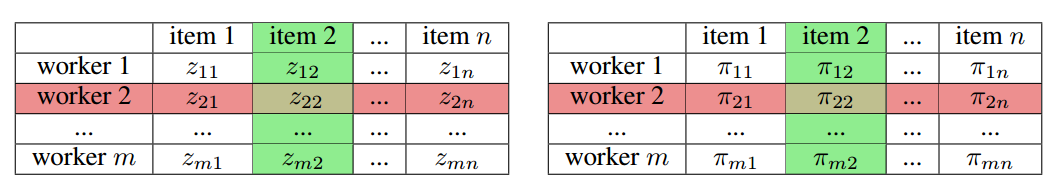
\includegraphics[width=0.95\columnwidth]{minimax_entropy.png}
  \caption{Left: observed labels. Right: underlying
    distributions. Highlights on both tables indicate that rows and
    columns of the distributions are constrained by sums over observations.}
  ~\label{fg:minimax_entropy_model}
\end{figure}

\subsection{Minimax Entropy}
\cite{Zhou2012-ry} proposed a minimax entropy principle to estimate
the ground truth given the observed labels by workers. The model is
illustrated in Figure~\ref{fg:minimax_entropy_model}. Each row
corresponds to a works indexed by $i$ (from 1 to $m$). Each column
corresponds to an item to be labeled, indexed by $j$ (from 1 to
$n$). Each item has an unobserved label represented as a vector
$y_{jl}$, which is 1 when item $j$ is in class $l$ (from 1 to $c$),
and 0 otherwise. Observed data is a tensor of labels $z_{ijk}$, which
is 1 when the item $i$ is labeled as class $j$ by the worker $i$, and
0 otherwise. We assume that $z_{ij}$ are drawn from
$\pi_{ij}$. $\pi_{ij}$ can be represented as a tensor $\pi_{ijk}$,
which is the probability that worker $i$ labels item $j$ as class
$k$. The proposed model will estimate $y_{jl}$ from the observed
$z_{ij}$.

The maximum entropy model for $\pi_{ij}$ given $y_{jl}$ is as
following:

\begin{align}
\max_{\pi} & -\sum_{i=1}^{m}\sum_{j=1}^{n}\sum_{k=1}^{c} \pi_{ijk}
\ln \pi_{ijk} \nonumber \\
  \mathrm{s.t.} & \sum_{i=1}^{m}\pi_{ijk} = \sum_{i=1}^{m}z_{ijk},
                  \forall j,k, ~ \sum_{j=1}^{n}y_{jl}\pi_{ijk} =
                  \sum_{j=1}^{n}y_{jl}z_{ijk} \forall i,k,l, \nonumber
  \\
  & \sum_{k=1}^{c}\pi_{ijk}=1, \forall i,j, \pi_{ijk} \geq 0, \forall
    i,j,k. \label{eq:max_entropy}
\end{align}

To infer $y_{jl}$, they proposed to choose $y_{jl}$ to minimize the
entropy in Equation~\ref{eq:max_entropy}.

\begin{align}
\min_{y}\max_{\pi} & -\sum_{i=1}^{m}\sum_{j=1}^{n}\sum_{k=1}^{c} \pi_{ijk}
\ln \pi_{ijk} \nonumber \\
  \mathrm{s.t.} & \sum_{i=1}^{m}\pi_{ijk} = \sum_{i=1}^{m}z_{ijk},
                  \forall j,k, ~ \sum_{j=1}^{n}y_{jl}\pi_{ijk} =
                  \sum_{j=1}^{n}y_{jl}z_{ijk} \forall i,k,l, \nonumber
  \\
  & \sum_{k=1}^{c}\pi_{ijk}=1, \forall i,j, \pi_{ijk} \geq 0, \forall
    i,j,k, \sum_{l=1}^{c}y_{jl}=1, \forall j, y_{jl} \geq 0, \forall
    j, l. \label{eq:minimax_entropy}
\end{align}

\section{Natural Language Processing for Enhancing Learning}
\subsection{Confusion Detector}
Given the enormous student/instructor ratio in a MOOC's discussion
forums, it is difficulty for an instructor to read all posts in a
MOOC's discussion forums. To address this issue, \cite{Agrawal2015-hp}
collected and created the Stanford MOOCPosts dataset: a corpus
composed of 29,604 anonymized learner forum posts from eleven Stanford
University public online classes. Each post in the MOOCPosts dataset
was scored across six dimensions -- confusion, sentiment, urgency,
question, answer, and opinion -- and subsequently augmented with
additional metadata. Then the authors built a confusion classifier from
the Stanford MOOCPost dataset to automatically detect confusion from
students posts and proposed a recommendation algorithm, which takes the
student confusion as input, to automatically recommended a
video lecture from a collection of several video lectures related to
the course.
\subsection{Automated Essay Scoring}
Automated grading is a critical part of Massive Open Online Courses (MOOCs) system and any intelligent tutoring systems (ITS) at scale. Essay writing is usually a common student assessment process in schools and universities. In this task, students are required to write essays of various length, given a prompt or essay topic. Some standard tests, such as Test of English as a Foreign Language (TOEFL) and Graduate Record Examination (GRE), assess student writing skills. Manually grading these essay will be time-consuming. Thus automated essay scoring (AES) systems has been used in these tests to reduce the time and cost of grading essays. Moreover, as massive open online courses (MOOCs) become widespread and the number of students enrolled in one course increases, the need for grading and providing feedback on written assignments are ever critical.

AES has employed numerous efforts to improving its performance. AES uses statistical and Natural Language Processing (NLP) techniques to automatically predict a score for an essay based on the essay prompt and rubric. Most existing AES systems are built on the basis of predefined features, e.g. number of words, average word length, and number of spelling errors, and a machine learning algorithm \cite{Chen2013-zw}. It is normally a heavy burden to find out effective features for AES. Moreover, the performance of the AES systems is constrained by the effectiveness of the predefined features. Recently another kind of approach has emerged, employing neural network models to learn the features automatically in an end-to-end manner \cite{Taghipour2016-ns}. By this means, a direct prediction of essay scores can be achieved without performing any feature extraction. The model based on long short-term memory (LSTM) networks in \cite{Taghipour2016-ns} has demonstrated promise in accomplishing multiple types of automated grading tasks.

\subsection{NLP in PeerAssist}
The goal of PeerAssist is to crowdsource the explanation (in the
format of texts) of how to solve a
given problem from students and apply multi-armed bandit algorithm to
efficiently select the most helpful and useful peer explanation from all collected
peer explanations for a given problem. The effectiveness of each peer
explanations is measured in three dimensions: teacher's rating (thumb
up or thumb down), student's rating (thumb up or thumb down), and the
student next problem correctness after receiving the peer explanation.
\bibliographystyle{apalike}
\bibliography{references}
\end{document}

%%% Local Variables:
%%% mode: latex
%%% TeX-master: t
%%% End:
